\section{Optimising Type Slice Calculation}
\label{sec:algorithms}

\providecommand{\tmslice}[2]{\mathit{TermMin}\;#1 \mathbin{\blacktriangleleft} #2}
\providecommand{\mintmslice}[2]{\mathit{MinTermMin}\;#1 \mathbin{\blacktriangleleft} #2}
\providecommand{\syntypeslice}[2]{\mathit{TypeSlice}^{\synmode}\;#1 \mathbin{\blacktriangleleft} #2}
\providecommand{\anatypeslice}[2]{\mathit{TypeSlice}^{\anamode}\;#1 \mathbin{\blacktriangleleft} #2}
\providecommand{\tmcalc}[5]{#1 \mathbin{{\color{BrickRed}\blacktriangleleft}} #2 \;{\color{BrickRed}\rightsquigarrow}\; #3 \mathbin{\synmode} #4 \,\dashv\, #5}
\providecommand{\tmrule}[7][\Delta;\,\Gamma]{%
  #1 \vdash #2 \mathbin{\synmode} #3
  \mathbin{{\color{BrickRed}\blacktriangleleft}} #4
  \;{\color{BrickRed}\rightsquigarrow}\; #5
  \mathbin{\synmode} #6
  \,\dashv\, #7%
}

\providecommand{\stkU}[2]{%
  \tikz[baseline=(N.base)]{%
    \node[inner sep=0pt, outer sep=0pt] (N) {\strut$#2$};%
    \foreach \col/\off in {#1}{%
      \draw[\col, line width=1.2pt, line cap=butt, overlay]
        ([xshift=-3pt,yshift=\off]N.south west) -- ([xshift=3pt,yshift=\off]N.south east);%
    }%
    \path ([yshift=-10pt]N.south west) ([yshift=-10pt]N.south east);%
  }%
}
\providecommand{\tokensp}{\mskip8mu}
\providecommand{\sABCD}[1]{\stkU{BrickRed/-1pt,NavyBlue/-3.4pt,OliveGreen/-5.8pt,Mulberry/-8.2pt}{#1}}
\providecommand{\sABC}[1]{\stkU{BrickRed/-1pt,NavyBlue/-3.4pt,OliveGreen/-5.8pt}{#1}}
\providecommand{\sABD}[1]{\stkU{BrickRed/-1pt,NavyBlue/-3.4pt,Mulberry/-8.2pt}{#1}}
\providecommand{\sAC}[1]{\stkU{BrickRed/-1pt,OliveGreen/-5.8pt}{#1}}
\providecommand{\sAD}[1]{\stkU{BrickRed/-1pt,Mulberry/-8.2pt}{#1}}
\providecommand{\sBC}[1]{\stkU{NavyBlue/-3.4pt,OliveGreen/-5.8pt}{#1}}
\providecommand{\sBD}[1]{\stkU{NavyBlue/-3.4pt,Mulberry/-8.2pt}{#1}}
\providecommand{\sC}[1]{\stkU{OliveGreen/-5.8pt}{#1}}
\providecommand{\sD}[1]{\stkU{Mulberry/-8.2pt}{#1}}
\providecommand{\sPone}[1]{\stkU{OliveGreen/-1pt}{#1}}
\providecommand{\sPtwo}[1]{\stkU{Mulberry/-3.4pt}{#1}}
\providecommand{\sPboth}[1]{\stkU{OliveGreen/-1pt,Mulberry/-3.4pt}{#1}}

\bigskip
\noindent The theory of synthesis and analysis slices (\S\ref{sec:synthesis}, \S\ref{sec:analysis}) establishes \textit{which} slices exist, and provides a brute-force algorithm. This section explores these structures further to improve the brute-force algorithm.

\subsection{Products of Synthesis Slices}
\label{sec:product-revisited}


We earlier suggested recursively calculating minimal slices of subterms and composing them together (\S\ref{sec:decompositions}). However, this cannot be done naively: the product of two minimal slices is not necessarily minimal. Consider the following if statement:
\[ \Gamma = (x \mathbin{:} \mathbf{1} \funarr \mathbf{1},\; y \mathbin{:} \mathbf{1} \funarr \mathbf{1}), \qquad e = \mathbf{if}\;\mathbf{true}\;\mathbf{then}\;x\;\mathbf{else}\;y, \qquad \tau = \mathbf{1} \funarr \mathbf{1}, \]
and ask for slices of $D : \synthesis{e}{\tau}$ at the full query $\upsilon = \mathbf{1} \funarr \mathbf{1}$. There are \textit{four} incomparable minimal full slices, displayed together as underlines:

\begin{center}
\begin{tikzpicture}[baseline=(t.base), every node/.style={inner sep=3pt}]
  \node[inner sep=0pt] (ax) {$x : \sAC{\mathbf{1}} \mathrel{\sABC{\funarr}} \sBC{\mathbf{1}}$};
  \node[inner sep=0pt, anchor=west] (xmark) at (ax.west) {$\phantom{x : }$};
  \node[inner sep=0pt, right=3.5em of ax] (ay) {$y : \sBD{\mathbf{1}} \mathrel{\sABD{\funarr}} \sAD{\mathbf{1}}$};
  \node[inner sep=0pt, anchor=west] (ymark) at (ay.west) {$\phantom{y : }$};
  \node[inner sep=0pt] at ($(ax.east)!0.3!(ay.west)$) {$,$};
  \node[draw, line width=0.9pt, rounded corners, fit=(ax)(ay),
        label={[font=\scriptsize\itshape]above:assumptions}] (a) {};
  \coordinate (col1) at (xmark.east |- a.south);
  \coordinate (col2) at ($(ax.east |- a.south) + (3pt,0)$);
  \coordinate (col3) at (ymark.east |- a.south);
  \node[font=\tiny\bfseries, BrickRed,   anchor=east, inner sep=1pt] at ([yshift=12pt]col1)  {(A)};
  \node[font=\tiny\bfseries, OliveGreen, anchor=east, inner sep=1pt] at ([yshift=7.2pt]col1) {(C)};
  \node[font=\tiny\bfseries, NavyBlue,   anchor=west, inner sep=1pt] at ([yshift=9.6pt]col2) {(B)};
  \node[font=\tiny\bfseries, NavyBlue,   anchor=east, inner sep=1pt] at ([yshift=9.6pt]col3) {(B)};
  \node[font=\tiny\bfseries, BrickRed,   anchor=west, inner sep=1pt] at ([yshift=12pt]a.south east)  {(A)};
  \node[font=\tiny\bfseries, Mulberry,   anchor=west, inner sep=1pt] at ([yshift=4.8pt]a.south east) {(D)};
  \node[right=5em of a] (t)
       {$\sABCD{\mathbf{if}}\tokensp\mathbf{true}\tokensp\sABCD{\mathbf{then}}\tokensp\sABC{x}\tokensp\sABCD{\mathbf{else}}\tokensp\sABD{y}$};
  \node[font=\tiny\bfseries, BrickRed,   anchor=east, inner sep=1pt] at ([yshift=12pt]t.south west)   {(A)};
  \node[font=\tiny\bfseries, NavyBlue,   anchor=west, inner sep=1pt] at ([yshift=9.6pt]t.south east)  {(B)};
  \node[font=\tiny\bfseries, OliveGreen, anchor=east, inner sep=1pt] at ([yshift=7.2pt]t.south west)  {(C)};
  \node[font=\tiny\bfseries, Mulberry,   anchor=west, inner sep=1pt] at ([yshift=4.8pt]t.south east)  {(D)};
\end{tikzpicture}
\end{center}

\begin{description}
\item[{\color{BrickRed}(A)}] Both branches are retained; the assumption slice keeps $x$'s domain only and $y$'s codomain only (joining to $1 \funarr 1$).
\item[{\color{NavyBlue}(B)}] Symmetric to (A), taking the opposite choices for the assumption slice
\item[{\color{OliveGreen}(C)}] \textbf{Else}-branch omitted.
\item[{\color{Mulberry}(D)}] Symmetric to (C): \textbf{then}-branch omitted.
\end{description}

Slices {\color{BrickRed}(A)} and {\color{NavyBlue}(B)} are minimal because each variable is sliced \textit{differently} across the two uses, and none are \textit{program} slices of each other. However, notice that {\color{BrickRed}(A)} and {\color{NavyBlue}(B)} are not subslices of the product with $x$, where only 2 minima exist:

\begin{center}
\begin{tikzpicture}[baseline=(t.base), every node/.style={inner sep=3pt}]
  \node[inner sep=0pt] (ax) {$x : \sPboth{\mathbf{1}\funarr\mathbf{1}}$};
  \node[inner sep=0pt, anchor=west] (xmark) at (ax.west) {$\phantom{x : }$};
  \node[inner sep=0pt, right=2.5em of ax] (ay) {$y : \sPtwo{\mathbf{1}\funarr\mathbf{1}}$};
  \node[inner sep=0pt, anchor=west] (ymark) at (ay.west) {$\phantom{y : }$};
  \node[inner sep=0pt] at ($(ax.east)!0.3!(ay.west)$) {$,$};
  \node[draw, line width=0.9pt, rounded corners, fit=(ax)(ay),
        label={[font=\scriptsize\itshape]above:assumptions}] (a) {};
  \coordinate (col1) at (xmark.east |- a.south);
  \coordinate (col2) at ($(ax.east |- a.south) + (3pt,0)$);
  \coordinate (col3) at (ymark.east |- a.south);
  \node[font=\tiny\bfseries, OliveGreen, anchor=east, inner sep=1pt] at ([yshift=12pt]col1)  {(C)};
  \node[font=\tiny\bfseries, Mulberry,   anchor=west, inner sep=1pt] at ([yshift=9.6pt]col2) {(D)};
  \node[font=\tiny\bfseries, Mulberry,   anchor=east, inner sep=1pt] at ([yshift=9.6pt]col3) {(D)};
  \node[right=5em of a] (t)
       {$\sPboth{(}\tokensp\sPboth{\mathbf{if}}\tokensp\mathbf{true}\tokensp\sPboth{\mathbf{then}}\tokensp\sPone{x}\tokensp\sPboth{\mathbf{else}}\tokensp\sPtwo{y}\tokensp\sPboth{\mathbf{,}}\tokensp\sPboth{x}\tokensp\sPboth{)}$};
  \node[font=\tiny\bfseries, OliveGreen, anchor=east, inner sep=1pt] at ([yshift=12pt]t.south west)  {(C)};
  \node[font=\tiny\bfseries, Mulberry,   anchor=west, inner sep=1pt] at ([yshift=9.6pt]t.south east) {(D)};
\end{tikzpicture}
\end{center}

When this expression is embedded in the product $(\mathbf{if}\;\mathbf{true}\;\mathbf{then}\;x\;\mathbf{else}\;y,\; x)$, the two assumptions are joined. However, the right projection's use of $x$ is strictly stronger than that of slices {\color{BrickRed}(A)}, {\color{NavyBlue}(B)}, and {\color{Mulberry}(D)}; we are \textit{aliasing} this variable's assumption. Slices {\color{BrickRed}(A)} and {\color{NavyBlue}(B)} are no longer minimal under this aliased assumption, meaning they are not subslices of the overall product. Slice {\color{Mulberry}(D)} is still valid because it does not actually use $x$.

\subsection{Term-Minimal Slices}
\label{sec:term-minimal-slices}

To rule out slices like (A) and (B) (\S\ref{sec:product-revisited}), we strengthen the notion of slices. We first calculate the minimal expression under \textit{maximal} typing assumptions, and then minimise the assumptions afterwards. By graduality, this is a minimal synthesis slice.

\begin{definition}[Term-minimal slice]
\label{def:term-minimal-slice}
A \textit{term-minimal slice} of $D : \synthesis{e}{\tau}$ on $\upsilon \in \lfloor \tau \rfloor$, written $\tmslice{D}{\upsilon}$, is a term slice $\varsigma \in \lfloor e \rfloor$ such that $\Delta;\,\Gamma \vdash \varsigma\;\synmode\;\psi$ for some $\psi \sqsupseteq \upsilon$ (with $\psi \in \lfloor \tau \rfloor$ by graduality, \cref{thm:graduality-syn}).
\end{definition}

Minimality lifts directly from the slice lattice on $e$ alone, and existence and monotonicity follow analogously to synthesis slices (\cref{thm:min-exists,thm:mono}).
\begin{definition}[Minimal Term-Minimal Slices]
\label{def:mintmslice}
A $\mintmslice{D}{\upsilon}$ is a $\tmslice{D}{\upsilon}$ minimal in $\tmslice{D}{\upsilon}$ under term-slice precision on $\lfloor e \rfloor$.
\end{definition}

Crucially, the two notions of minimality do not coincide: term-minimality is strictly stronger. Not all minimal slices are term-minimal under maximal assumptions.

\begin{counterexamplebox}
%
\begin{counterexample}[Minimal $\not\Rightarrow$ Term-Minimal]\label{lem:min-not-tmin}
Slices (A) and (B) (\S\ref{sec:product-revisited}) are minimal synthesis slices but are \textbf{not} term-minimal.
\end{counterexample}
\end{counterexamplebox}

\subsection{Calculating Term-Minimal Slices}
\label{sec:term-minimal-calculus}
The rest of this section develops a structural calculus that characterises minimal term slices via a judgement:
\[ \Gamma \vdash e \mathbin{\synmode} \tau \mathbin{\blacktriangleleft} \upsilon \;{\color{BrickRed}\rightsquigarrow}\; \varsigma \mathbin{\synmode} \psi \dashv \gamma, \]
read ``the typing $\Gamma \vdash e \synmode \tau$ at query $\upsilon$ produces term slice $\varsigma$, synthesises $\psi$, and uses assumptions $\gamma$''. The fourth output $\gamma$ is a minimal assumption slice to retrieve a minimal slice corresponding to the term-minimal slice.

\noindent The cases that deserve commentary are products, the binding constructs, function application, and type application; the \synr{Lam{:}}\ and \synr{Let}\ rules each carry a body re-typing premise (rightmost) which re-derives the body's typing under the binder slice $\gamma(x)$.

\subsubsection{Products}
With term minimality, we now have that two minimal synthesis slices which are also term-minimal can be composed into a term-minimal, minimal synthesis slice. For a query $\upsilon_1\times \upsilon_2$ on the product, the projections are queried with $\upsilon_1$ and $\upsilon_2$ individually:

\[
\inference[\synr{Pair}]{
  \tmrule{e_1}{\tau_1}{\upsilon_1}{\varsigma_1}{\psi_1}{\gamma_1}
  &
  \tmrule{e_2}{\tau_2}{\upsilon_2}{\varsigma_2}{\psi_2}{\gamma_2}
}{\tmrule{(e_1, e_2)}{\tau_1 \times \tau_2}{\upsilon_1 \times \upsilon_2}{(\varsigma_1, \varsigma_2)}{\psi_1 \times \psi_2}{\gamma_1 \sqcup \gamma_2}}
\]

\subsubsection{Function Application}
\label{sec:term-min-app}

All the synthesised type information from a function application is derived from the function itself. We may simply omit the argument, and slice the function by $\gap \funarr \upsilon$:
\[
\inference[\synr{App}]{
  \analysis{e_2}{\tau_1}
  &
  \upsilon \neq \gap
  &
  \tmrule{e_1}{\tau_1 \funarr \tau_2}{\gap \funarr \upsilon}{\varsigma_{\mathit{fn}}}{\psi_1}{\gamma}
}{\tmrule{e_1\,e_2}{\tau_2}{\upsilon}{\varsigma_{\mathit{fn}}(\gap)}{\mathsf{cod}(\psi_1)}{\gamma}}
\]

\subsubsection{Binding Constructs}
\label{sec:term-min-binders}

Rules which bind variables are more complex, as they abstract a variable used in the minimised body. The general method is to slice them by first slicing the \textit{body}, extracting the assumption it needed on the bound variable from the minimal assumptions $\gamma$, then slice the definition / type annotation using this. 

Notice that this is the \textit{opposite} direction to typechecking, e.g. let bindings type the definition first, then use the result to type the body, but slicing slices the body first to determine the minimal assumption to slice the definition with.

\subsubsection{Type Application}
\label{sec:term-min-tapp}

Type application works by matching the type function's type against the query to collect a list of constraints on the type variable, the \textit{join} of which gives the sliced type argument $\hat\sigma$. The type function is then sliced with a matched query $\widehat{\upsilon}$, where each position corresponding to the type variable $\alpha$ in the type function's type is replaced by $\alpha$ itself and other positions are carried over from the query unchanged. Figure~\ref{fig:tapp-minsub} illustrates the construction on a query whose two subparts are matched with an $\alpha$ with differing constraints.

\begin{figure}[H]
\centering
$e \mathbin{\synmode} \forall\alpha.\,(\alpha \times \alpha \times \mathbf{Bool})$,\quad applied at\quad $\sigma = \mathbf{1} \funarr (\mathbf{Bool} \times \mathbf{Bool})$:

\medskip

So $e\langle\sigma\rangle \mathbin{\synmode} (\mathbf{1} \funarr (\mathbf{Bool} \times \mathbf{Bool})) \times (\mathbf{1} \funarr (\mathbf{Bool} \times \mathbf{Bool})) \times \mathbf{Bool}$.

\medskip

\begin{tabular}{r@{\;\;}l}
\textbf{Query}             & $\upsilon \;=\; \underbrace{\sli[teal]{\mathbf{1} \funarr \gap}}_{\alpha} \;\times\; \underbrace{\sli[teal]{\gap \funarr (\mathbf{Bool} \times \gap)}}_{\alpha} \;\times\; \gap$ \\[16pt]
\textbf{Matched query}     & $\widehat{\upsilon} \;=\; \alpha \;\times\; \alpha \;\times\; \gap$ \\[8pt]
\textbf{Constraints}       & $\mathbf{1} \funarr \gap \;\sqsubseteq\; \alpha \qquad \gap \funarr (\mathbf{Bool} \times \gap) \;\sqsubseteq\; \alpha$ \\[8pt]
\textbf{Constraints Join}  & $\hat\sigma \;=\; \mathbf{1} \funarr (\mathbf{Bool} \times \gap)$ \\
\end{tabular}
\caption{Type application query constraints.}
\label{fig:tapp-minsub}
\end{figure}

\subsection{Case Expressions}
\label{sec:fixed-point}

The case rule is the difficult one, appearing to require an iterative fixed point algorithm. This is because the two branch types join to produce the resulting type which is being queried upon. As synthesis slices are not exact, a query may be split into two disjoint types, yet a minimal slice of one branch may produce a more precise type than the query (overflow), which is also produced by a sibling branch. The sibling branch may then admit further slicing, as it no longer needs to provide this redundant part of the type. Lack of an upwards version of monotonicity (\cref{fig:syn-slice-refinement}) makes this difficult to solve in general without brute force.

However, when the branch slices exactly synthesise disjoint type queries, then there is no redundancy and the result is minimal. The scrutinee can be sliced using the join of the minimal assumptions on the branches, much like with let bindings. 

To express disjoint types we can use \textit{co-Heyting subtraction} $\upsilon_1 \heytingminus \upsilon_2$, which is the least slice whose join with $\upsilon_2$ recovers $\upsilon_1$, i.e. ``the part of $\upsilon_1$ not already covered by $\upsilon_2$'', e.g. $\sli{1 \times 1} \;\heytingminus\; \sli{1 \times}\,\gap \;=\; \gap\,\sli{\times 1}$.

Then, a disjoint cover of query $\upsilon$ is one such that $\upsilon\heytingminus \upsilon_1 = \upsilon_2$ and $\upsilon \heytingminus \upsilon_2 = \upsilon_1$. The case expression will necessarily synthesise $\upsilon_1 \sqcup \upsilon_2$ which equals $\upsilon$ by standard co-Heyting algebra rules. Note that the lattice is \textit{not} a boolean algebra, so $\upsilon_1 \sqcap \upsilon_2 \neq \gap$ in general.

The Hazel implementation simply does a disjoint split and ignores the overflow issue to work in linear time complexity. This is why it is an approximation. But, it is perfectly feasible to use this approximation and then continue with the brute force algorithm, as we expect the approximation to be very close to the minimum in almost all cases. Further, as overflow only occurs due to variable aliasing, the brute force search need only consider aliased variables at the leaves.

\subsection{Calculating Analysis Slices}
\label{sec:ana-slice-calculus}

Analysis slices are calculated directly from synthesis slices. The only rule that creates a type checking judgement is function application. Consider the analysis slice of a function argument with query type $\upsilon_1$; it is just the function application and a slice of the function under $\gap \to \upsilon_1$. That is, to explain why a function argument must be a given type, we ask why the corresponding function has that type as its domain.

However, to recursively calculate the analysis slice of an application when the focus is deep inside the argument, the analysis slice of the argument itself must be calculated, but its outer derivation mode is in \textit{analysis}. The analysis slices defined earlier (\S\ref{sec:ana-slice-def}) do not apply here.

We need an additional notion of \textit{inner} analysis slices. Dually to regular (outer) analysis slices, which treat the synthesis mode as an \textit{input}, the inner slices treat the analysis derivation mode as an \textit{output}, and attempt to minimise it. 

Intuitively, an inner analysis slice gives the minimal assumptions, context, and additionally the minimum \textit{analysis type} to be imposed on it by the outer context, such that the queried analysis type holds at its focus. In particular, slicing the function in an application would use this minimal outer analysis mode type on the argument to slice the domain type of the function.
\vspace{-0.5em}
\begin{definition}
\label{def:ana-pos-slice}
An \textit{inner analysis slice} of $\mathit{Cls} : \ctxclass{\C}{\anamode\,\tau_p}{\Delta';\,\Gamma'}{\anamode\,\tau}$ on $\upsilon \in \lfloor\tau\rfloor$, written $\anaposslice{\mathit{Cls}}{\upsilon}$, is a triple $(\kappa, \gamma, \upsilon_{\mathrm{outer}}) \in \lfloor\C, \Gamma, \tau_p\rfloor$ such that $\ctxclass[\Delta;\,\gamma]{\kappa}{\anamode\,\upsilon_{\mathrm{outer}}}{\Delta'';\,\Gamma''}{\anamode\,\phi}$ for some inner-type witness $\phi \sqsupseteq \upsilon$ (with $\phi \in \lfloor\tau\rfloor$ by graduality, \cref{thm:graduality-ana-cls}).
\end{definition}
\vspace{-0.5em}

\section{Full Type Slices -- Slicing Assumption Definitions}
\label{sec:full-slices}
Synthesis slices are explained using a set of \textit{minimal assumptions}. However, in real code, these are actually \textit{provided by the surrounding context} (or from external code). Providing these minimal assumptions via a full slice of this context can be very meaningful. For example, when debugging a type error, the error itself may be \textit{non-local}, within a variable definition elsewhere, giving one of the used variables the wrong type. In this situation the error is in the definition, and we could debug it by inspecting (and slicing) that definition.

A \textit{full type slice} is a fully sliced decomposition of a program around a focus, which can be pieced back together to form a well-typed program with the same (or stronger) typing properties at the focus as some given query:

\vspace{-0.5em}
\begin{definition}[Type slices]
  \label{def:type-slice}
A \textit{type slice} of $\mathit{Cls} : \ctxclass{\C}{\synmode\,\tau_p}{\Delta';\,\Gamma'}{\synmode\,\tau}$ and $D : \synthesis[\Delta';\,\Gamma']{e}{\tau}$ on $\upsilon \in \lfloor\tau\rfloor$, written $\syntypeslice{(\mathit{Cls},D)}{\upsilon}$, is a pair $((\kappa,\gamma),(\gamma_f,\varsigma)) \in \lfloor\C,\Gamma\rfloor \times \lfloor\Gamma',e\rfloor$ such that $(\gamma_f,\varsigma) : \synslice{D}{\upsilon}$, and $\ctxclass[\Delta;\,\gamma]{\kappa}{\synmode\,\psi}{\Delta';\,\gamma_f'}{\synmode\,\phi'}$ for some $\psi$, and $\gamma_f' \sqsupseteq \gamma_f$ such that $\synthesis[\Delta';\ \gamma_f']{\varsigma}{\phi'}$.
\end{definition}
\vspace{-0.5em}

Importantly, the pair of slices forms a well-typed program: by context typing soundness, $\kappa[\varsigma]$ synthesises $\psi$. Then, a \textit{minimal} type slice is one in which the context $\kappa$ and the focused expression $\varsigma$ are jointly minimised alongside minimal external typing assumptions of the context typing $\gamma$. Notably, we do \textit{not} minimise the assumptions to the focused term, as its assumptions are now explicitly provided by the surrounding context (and $\gamma$).

As slices can be inexact, efficiently calculating a minimal context providing sufficient assumptions to a minimal \textit{SynSlice} at the focus is non-trivial. The Hazel implementation instead closely approximates this by slicing the definition / annotation on each binding by its required type as per the minimal assumptions of the focused term. When each slice of these definitions is exact, the resulting type slice is minimal.

For terms in analysis mode, the full type slice is just the analysis slice, as the empty focus (with type $\gap$) analyses successfully against any type.
\section{Minimum-Size Slices}
\label{sec:min-size}

Minimal slices are not unique, and some are actually larger than others in the sheer number of terms highlighted. So, one might rank them by \textit{size}: the number of highlighted positions, asking for a \textit{minimum-size} slice. For this core calculus, finding such a slice is \textbf{NP-hard} in general. 

We can construct a reduction from the NP-hard set cover optimisation problem as follows, and shown in \cref{fig:nphard}:
\begin{itemize}
  \item Encode a universe $U = \{1,\dots,n\}$ as a type $\tau = 1 \times \cdots \times 1$ ($n$ factors, one position per element)
\item Encode each of $m$-many sets $S_j$ in the set cover problem by an assumption $x_j : T_j \sqsubseteq \tau$ in $\Gamma$ with $T_j$ defined by the $i$th projection of $T_j$ being $1$ if and only if $i \in S_j$.
\item Construct a case tree with empty scrutinees and placing all $(x_j, I_j)$, defining $I_j$ as the $m$-ary product with $j$th projection being $1$ and all others $\gap$.
\end{itemize}

Then, if a synthesis slice is queried on this case tree with $\tau \times 1 \times \dots \times 1$, each $I_j$ must be retained, so the whole tree structure must be retained, and the only variance in the size of the slices is purely dependent on which variables $x_j$ were retained.

As we queried $\tau$ in the first projection then $\bigsqcup_{j=1}^m{T_j} = \tau$, which implies there are $m$ subsets\footnote{Subsets, as a minimal slice can use less precise assumptions $x_j$, i.e. $x_j : T'_j \sqsubseteq T_j$} $S_j' \subseteq S_j$ such that $\bigcup_{j=1}^mS'_j = U$. Hence, the retained $S_j$ form a set-cover. Finally, the only variance in the size of the slice was in the number of variables $x_j$ chosen, i.e. the number of sets chosen; hence, a minimum-size synthesis slice corresponds to a minimum set cover.

\begin{figure}[ht]
\centering
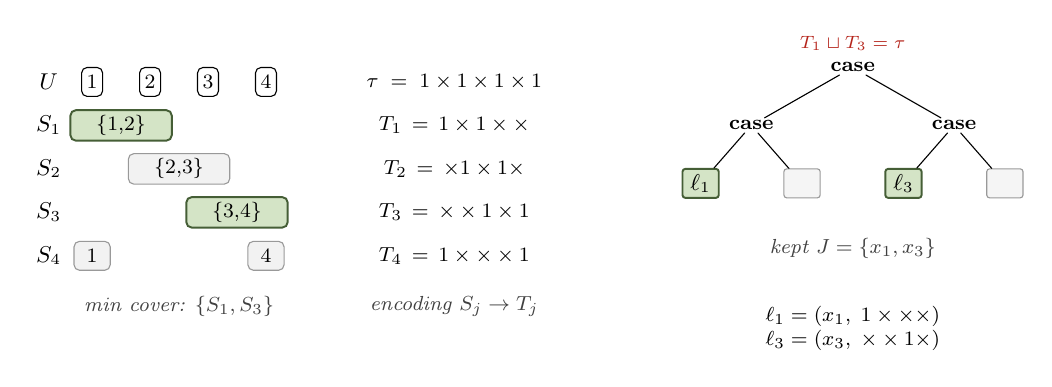
\begin{tikzpicture}[scale=0.92, transform shape,
    sc/.style={draw, rounded corners=2pt, inner sep=2pt, minimum height=4mm, font=\footnotesize},
    sel/.style={fill=OliveGreen!18, draw=OliveGreen!60!black, line width=0.7pt},
    no/.style={fill=black!5, draw=black!40},
    ca/.style={font=\bfseries\footnotesize, inner sep=1pt},
    lf/.style={draw, rounded corners=1pt, inner sep=2pt, minimum width=5mm, minimum height=4mm, font=\small},
    kp/.style={draw=OliveGreen!60!black, fill=OliveGreen!18, line width=0.7pt},
    dr/.style={draw=black!40, fill=black!4, text=black!50},
    every node/.append style={font=\small},
    line cap=round]

\node[font=\itshape\small] at (-0.6,0.6) {$U$};
\node[sc] at (0.0,0.6) {1};
\node[sc] at (0.8,0.6) {2};
\node[sc] at (1.6,0.6) {3};
\node[sc] at (2.4,0.6) {4};

\node[font=\itshape\small] at (-0.6,0.0) {$S_1$};
\node[sc, sel, minimum width=14mm] at (0.4,0.0) {\{1,2\}};
\node[font=\itshape\small] at (-0.6,-0.6) {$S_2$};
\node[sc, no,  minimum width=14mm] at (1.2,-0.6) {\{2,3\}};
\node[font=\itshape\small] at (-0.6,-1.2) {$S_3$};
\node[sc, sel, minimum width=14mm] at (2.0,-1.2) {\{3,4\}};
\node[font=\itshape\small] at (-0.6,-1.8) {$S_4$};
\node[sc, no,  minimum width=5mm]  at (0.0,-1.8) {1};
\node[sc, no,  minimum width=5mm]  at (2.4,-1.8) {4};

\node[font=\footnotesize\itshape, text=gray!50!black, align=center] at (1.2,-2.5)
  {min cover: $\{S_1,S_3\}$};

\node[font=\footnotesize, align=left] at (5.0,0.6)  {$\tau \;=\; 1 \times 1 \times 1 \times 1$};
\node[font=\footnotesize, align=left] at (5.0,0.0)  {$T_1 \,=\, 1 \times 1 \times \gap \times \gap$};
\node[font=\footnotesize, align=left] at (5.0,-0.6) {$T_2 \,=\, \gap \times 1 \times 1 \times \gap$};
\node[font=\footnotesize, align=left] at (5.0,-1.2) {$T_3 \,=\, \gap \times \gap \times 1 \times 1$};
\node[font=\footnotesize, align=left] at (5.0,-1.8) {$T_4 \,=\, 1 \times \gap \times \gap \times 1$};
\node[font=\footnotesize\itshape, text=gray!50!black, align=center] at (5.0,-2.5)
  {encoding $S_j \to T_j$};

\node[ca] (rt) at (10.5, 0.8) {case};
\node[ca] (cl) at ( 9.1, 0.0) {case};
\node[ca] (cr) at (11.9, 0.0) {case};
\node[lf, kp] (l1) at ( 8.4,-0.8) {$\ell_1$};
\node[lf, dr] (l2) at ( 9.8,-0.8) {$\gap$};
\node[lf, kp] (l3) at (11.2,-0.8) {$\ell_3$};
\node[lf, dr] (l4) at (12.6,-0.8) {$\gap$};
\draw (rt) -- (cl);
\draw (rt) -- (cr);
\draw (cl) -- (l1);
\draw (cl) -- (l2);
\draw (cr) -- (l3);
\draw (cr) -- (l4);
\node[font=\scriptsize, text=BrickRed, anchor=south] at (rt.north) {$T_1 \sqcup T_3 = \tau$};
\node[font=\footnotesize\itshape, text=gray!50!black, align=center] at (10.5,-1.7)
  {kept $J = \{x_1, x_3\}$};
\node[font=\footnotesize, align=center] at (10.5,-2.8)
  {$\ell_1 = (x_1,\; {1} \times \gap \times \gap \times \gap)$\\
   $\ell_3 = (x_3,\; \gap \times \gap \times {1} \times \gap)$};
\end{tikzpicture}
\caption{NP-Hardness of Minimum-Size Slicing}
\label{fig:nphard}
\end{figure}



%%% Local Variables:
%%% mode: LaTeX
%%% TeX-master: "PolymorphicTypeSlicing"
%%% End:
